\documentclass{article}

% if you need to pass options to natbib, use, e.g.:
%     \PassOptionsToPackage{numbers, compress}{natbib}
% before loading neurips_2026

% The authors should use the "dblblindworkshop" option for the Workshop with double-blind reviewing
\usepackage[dblblindworkshop]{neurips_2026}

% "preprint" option is used for arXiv or other preprint submissions
% \usepackage[preprint]{neurips_2026}

% to avoid loading the natbib package, add option nonatbib:
%    \usepackage[nonatbib]{neurips_2026}


% After being accepted, the authors should uncomment the following line to compile a camera-ready version.
% \usepackage[dblblindworkshop, final]{neurips_2026}

\workshoptitle{I Can't Believe It's Not Better (ICBINB): Failure Modes of AI in Biology}


\usepackage[utf8]{inputenc} % allow utf-8 input
\usepackage[T1]{fontenc}    % use 8-bit T1 fonts
\usepackage{hyperref}       % hyperlinks
\usepackage{url}            % simple URL typesetting
\usepackage{booktabs}       % professional-quality tables
\usepackage{amsfonts}       % blackboard math symbols
\usepackage{nicefrac}       % compact symbols for 1/2, etc.
\usepackage{microtype}      % microtypography
\usepackage{xcolor}         % colors
\usepackage{graphicx}

% Note. For the workshop paper template, both \title{} and \workshoptitle{} are required, with the former indicating the paper title shown in the title and the latter indicating the workshop title displayed in the footnote. 
\title{Confidence Does Not Make Proteins:\\
Reward Hacking in pLDDT-Guided Preference Optimization}


% The \author macro works with any number of authors. There are two commands
% used to separate the names and addresses of multiple authors: \And and \AND.
%
% Using \And between authors leaves it to LaTeX to determine where to break the
% lines. Using \AND forces a line break at that point. So, if LaTeX puts 3 of 4
% authors names on the first line, and the last on the second line, try using
% \AND instead of \And before the third author name.


\author{%
  David S.~Hippocampus\thanks{Use footnote for providing further information
    about author (webpage, alternative address)---\emph{not} for acknowledging
    funding agencies.} \\
  Department of Computer Science\\
  Cranberry-Lemon University\\
  Pittsburgh, PA 15213 \\
  \texttt{hippo@cs.cranberry-lemon.edu} \\
  % examples of more authors
  % \And
  % Coauthor \\
  % Affiliation \\
  % Address \\
  % \texttt{email} \\
  % \AND
  % Coauthor \\
  % Affiliation \\
  % Address \\
  % \texttt{email} \\
  % \And
  % Coauthor \\
  % Affiliation \\
  % Address \\
  % \texttt{email} \\
  % \And
  % Coauthor \\
  % Affiliation \\
  % Address \\
  % \texttt{email} \\
}


\begin{document}


\maketitle


\begin{abstract}
Instruction tuning can teach a language model to generate protein sequences
that follow requested physicochemical properties, but it does not directly
optimize structural quality. We tested whether direct preference optimization
(DPO) using ESMFold pLDDT as the preference signal could close this gap in one
protein family. In a matched evaluation on 260 held-out prompts, self-play DPO
raised mean pLDDT from 49.0 to 67.9. The apparent improvement, however, was a failure:
the fraction of generations satisfying the specification fell from 19.2\% to
1.2\%, the fraction passing sequence-plausibility filters fell from 88.8\% to
27.3\%, and only 1 of 260 self-play outputs passed both criteria and pLDDT $\geq 70$.
The policy produced long, lysine-rich, low-complexity sequences with extreme
positive charge. DPO reward accuracy remained high because the implicit
rewards of the preferred and rejected responses declined together while their
margin increased. A bundled repair that used natural proteins as preferred
responses and added a supervised likelihood term restored plausibility. In a second matched run,
repeating the repair with fresh negatives did not improve the joint endpoint. These results show that improving
predictor confidence can move a generative policy away from the intended
biological task, and that the remedy need not support continued iteration.
\end{abstract}



\section{Introduction}
Autoregressive protein language models can generate diverse amino-acid
sequences and can be adapted to specific families or design objectives
\citep{ferruz2022protgpt2,nijkamp2023progen2}. Instruction tuning offers a
direct interface: a user describes desired properties, and the model generates
a sequence intended to satisfy them. In our system, supervised fine-tuning
(SFT) substantially improved compliance with requested properties. Predicted structural confidence, however, remained low.

A natural next step is to optimize against a structure predictor. ESMFold
predicts a structure from a single sequence and reports per-residue confidence
through pLDDT \citep{lin2023esmfold}. DPO can then prefer model outputs with
higher pLDDT without fitting a separate reward model
\citep{rafailov2023dpo}. Closely related work has used AlphaFold pLDDT as a
preference signal for fixed-backbone protein design
\citep{xue2025residpo}. The central assumption is that increasing predictor
confidence will increase the frequency of useful sequences while preserving
the behavior learned during SFT.

Here, we report a case in which such an assumption fails. On a held-out slice from the
PF00416 ribosomal-protein family, self-play DPO sharply increased pLDDT by
learning a shortcut: long, low-complexity, positively charged sequences that
ESMFold scored confidently but that no longer satisfied the requested
properties. This is reward hacking in the operational sense that optimizing a
proxy reduces performance on the intended objective
\citep{skalse2022reward}. We then tested a repair in which the preferred
response was a natural protein rather than another model sample. The repair
partially recovered useful generations, but a second round with fresh,
harder negatives produced no further improvement.

The paper makes three empirical contributions. First, it documents the full
trajectory from successful instruction tuning to proxy optimization and
behavioral collapse under a matched evaluation. Second, it identifies the
sequence shortcut and shows why reward accuracy did not diagnose the failure.
Third, it reports both a partial repair and a matched negative result for
repeating that repair. Overall, the results suggest that predicted structural
confidence, instruction compliance, and sequence plausibility must be measured
together.

\section{Problem}
\label{sec:problem}

\paragraph{Task and evaluation.}
We instruction-tuned Llama-3.1-8B-Instruct
\citep{grattafiori2024llama3}, using 4-bit QLoRA
\citep{hu2022lora,dettmers2023qlora} on 348{,}867 prompt-sequence pairs from
reviewed UniProtKB entries \citep{uniprot2023}. Prompts described a subset of
properties computed from the natural sequence, including length, net charge at
pH 7.4, hydrophobicity, stability, aggregation propensity, cysteine count, and
protein family. The data were split by MMseqs2 clusters at 30\% sequence
identity and 80\% coverage \citep{steinegger2017mmseqs2}. The supervised stage was trained and evaluated across this multi-family corpus and improved adherence across the directly recomputable properties substantially (Appendix Figure~\ref{fig:papera-adherence}), confirming that the model learned to follow the requested specifications. Nevertheless, predicted structural confidence remained suboptimal overall and was not directly optimized during SFT (Figure ~\ref{fig:story}a). We therefore selected PF00416, the ribosomal-protein uS13 family, as a controlled testbed for investigating whether pLDDT-guided preference optimization could improve structural confidence without compromising instruction adherence.

\paragraph{What counts as success?}
To determine whether DPO improved the intended task rather than merely the optimized proxy, we evaluated the resulting sequence generations along three dimensions (Table~\ref{tab:criteria-simple}): First, is it \emph{on specification}: does it meet every property stated in the prompt and remain within the family's length and
charge ranges? Second, is it \emph{protein-like}: does it pass inexpensive
sequence checks for low complexity, residue imbalance, tandem repetition,
minimum length, and canonical amino acids? Third, does ESMFold assign high
predicted confidence, defined as mean pLDDT $\geq 70$? The exact gate and filter
definitions are given in Appendix~\ref{app:criteria}. 

\begin{table}[t]
\caption{The evaluation separates the optimized proxy from the intended task.
The primary endpoint requires all three criteria.}
\label{tab:criteria-simple}
\centering
\small
\setlength{\tabcolsep}{5pt}
\begin{tabular}{@{}lll@{}}
\toprule
Criterion & Question & Operational definition \\
\midrule
On specification (Gate) & Does it follow the request? & All prompt constraints and family bounds pass \\
Protein-like (Filter) & Is the sequence plausible? & All sequence-only filters pass \\
High confidence & Is the prediction confident? & Mean ESMFold pLDDT $\geq 70$ \\
\midrule
Passes all three & Is it a useful computational hit? & Conjunction of the three rows above \\
\bottomrule
\end{tabular}
\end{table}

%This definition deliberately does not call a generation a folded protein. pLDDT is a predictor-confidence score, not experimental evidence of folding or function \citep{jumper2021alphafold,lin2023esmfold}. The question tested here is narrower: can pLDDT-based preference optimization increase the number of generations that are simultaneously on specification, protein-like, and assigned high confidence?

\section{Proposed approach}
\label{sec:approach}
\paragraph{Preference-optimization setup.}
Starting from the SFT checkpoint, we used preference optimization as a post-training step for improving predicted structural confidence within PF00416. The available family slice comprised 571 natural sequences, of which 311 were assigned to training and 260 were held out for evaluation; preference pairs were constructed exclusively from the training split. DPO learns from two responses to the same prompt: one designated as preferred and the other as rejected. ESMFold pLDDT was used to construct preference labels. 

\paragraph{Self-play DPO.}
Our first approach constructed both sides of each preference pair from the SFT model’s own generations. For each PF00416 training prompt, we sampled multiple candidate sequences and discarded those that failed the specification gate or sequence-sanity filters. The remaining candidates were evaluated with ESMFold, and higher-pLDDT generations were paired as preferred responses with lower-pLDDT generations from the same prompt. This procedure yielded 859 preference pairs from 310 unique training prompts. We call this procedure self-play DPO because both the preferred and rejected responses were produced by the policy. We trained a LoRA adapter with DPO ($\beta=0.3$) while holding the SFT policy fixed as the reference. The hypothesis was that the model would shift probability toward its more confidently predicted generations without losing instruction-following behavior.

\paragraph{Natural-positive anchoring.}
After completing the self-play experiment, we evaluated a second preference construction intended to anchor the update to the natural sequence distribution. For each prompt, the associated natural training sequence served as the preferred response, while a model-generated sequence served as the rejected response. The anchored round-1 dataset contained 929 preference pairs from 310 unique training prompts. We also increased the DPO coefficient to $\beta=0.5$ and added a negative-log-likelihood term on the natural response with weight $\alpha=1$. We refer to this combined intervention as anchored DPO.

\paragraph{Iterating anchored DPO.}
Anchored round 1 used negatives sampled from the SFT policy. To test whether the procedure could support iterative refinement, round 2 initialized from the round-1 policy, sampled fresh negatives from that policy, and applied the same anchored objective, yielding 906 preference pairs from 303 unique training prompts. The round-1 checkpoint was re-evaluated alongside round 2 in the same generation process to provide a matched comparison. All policy evaluations used one sampled generation ($K=1$) for each of the 260 held-out prompts, and comparisons were restricted to policies generated within the same evaluation block. Hyperparameters and the complete evaluation protocol are reported in Appendix~\ref{app:protocol}.

\section{Observed outcome}
\label{sec:outcome}

\subsection{Instruction tuning improves adherence, not pLDDT}

On PF00416, the base model produced no on-spec outputs among 260 held-out generations. After SFT, the on-spec rate increased to 19.2\%, while the sequence-sanity-filter pass rate increased from 24.6\% to 88.8\% (Table~\ref{tab:results}, block A). Predicted structural confidence did not improve: mean pLDDT was 51.1 for the base model and 49.0 after SFT. Thus, SFT improved instruction adherence and basic sequence sanity but left the structural-confidence problem unresolved.

\begin{figure}[t]
\centering
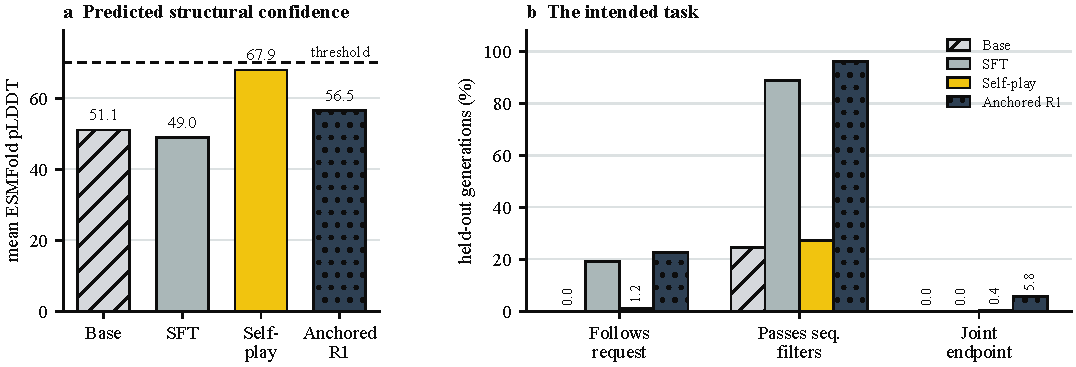
\includegraphics[width=\linewidth]{figures/fig1_linear_story.pdf}
\caption{Self-play improves the proxy and damages the intended task.
All values come from evaluation block A: one generation for each of the same
260 held-out prompts, produced and evaluated in one process. Percentages use
260 as the denominator. Mean pLDDT excludes unparseable outputs. The
specification gate includes both requested properties and unconditional family
bounds; the primary endpoint requires the specification gate, all plausibility
filters, and pLDDT $\geq70$.}
\label{fig:story}
\end{figure}

\subsection{Self-play raises pLDDT by leaving the intended task}

Self-play DPO raised mean pLDDT from 49.0 to 67.9
(Figure~\ref{fig:story}a). Taken alone, the optimized metric indicated a large
improvement. The remaining measurements, however, showed the opposite. The on-spec rate fell from 19.2\% to 1.2\%, and the protein-like rate fell from 88.8\% to
27.3\% (Figure~\ref{fig:story}b). The primary endpoint remained essentially
zero: SFT produced 0 joint successes and self-play produced 1 among 260
prompts.

The failure was also apparent in basic sequence properties. Mean length rose
from 138 to 350 residues, although natural PF00416 sequences had mean length
123 in the available reference set. For prompts that requested charge, mean
absolute charge error rose from 6.6 to 103.0. The model had become substantially
better at obtaining ESMFold confidence and substantially worse at the task for
which it had been instruction-tuned.

\begin{table}[t]
\caption{Two matched held-out evaluations. Each block contains models
generated and evaluated together on the same 260 prompts ($K=1$). ``All three'' gives count and percentage. pLDDT and length exclude
unparseable outputs; Charge MAE is the mean absolute difference between the requested and recomputed net charge at pH 7.4.}
\label{tab:results}
\centering
\small
\setlength{\tabcolsep}{3.1pt}
\begin{tabular}{@{}lrrrrrr@{}}
\toprule
System & pLDDT & On-spec & Protein-like & All three & Length & Charge MAE \\
\midrule
\multicolumn{7}{@{}l}{\textit{A. Failure and first repair, evaluated together}} \\
Base & 51.1 & 0.0\% & 24.6\% & 0 (0.0\%) & 425 & 34.2 \\
SFT & 49.0 & 19.2\% & 88.8\% & 0 (0.0\%) & 138 & 6.6 \\
Self-play DPO & \textbf{67.9} & 1.2\% & 27.3\% & 1 (0.4\%) & 350 & 103.0 \\
Anchored DPO, R1 & 56.5 & \textbf{22.7\%} & \textbf{96.2\%} & \textbf{15 (5.8\%)} & 130 & \textbf{4.0} \\
\midrule
\multicolumn{7}{@{}l}{\textit{B. Second-round test, with R1 re-evaluated alongside R2}} \\
SFT & 49.4 & 16.9\% & 88.5\% & 1 (0.4\%) & 145 & 8.5 \\
Anchored DPO, R1 & \textbf{57.6} & 25.8\% & 96.5\% & \textbf{19 (7.3\%)} & \textbf{128} & \textbf{3.5} \\
Anchored DPO, R2 & 56.8 & \textbf{26.2\%} & \textbf{96.9\%} & 16 (6.2\%) & 135 & 4.8 \\
\bottomrule
\end{tabular}
\end{table}

\subsection{Natural-positive anchoring partially repairs the failure}

In evaluation block A, anchored round 1 recovered a 96.2\% protein-like rate
and increased the on-spec rate to 22.7\%. Mean length returned to 130 residues,
and charge MAE fell to 4.0. Most importantly, the number passing all three
criteria rose from 0/260 for SFT to 15/260 (5.8\%; 95\% Wilson interval
3.5-9.3\%). In the paired comparison, 15 prompts succeeded only under anchored R1, whereas none succeeded only under SFT.
The repair was meaningful but incomplete: 245 of 260 generations still failed
the primary endpoint.

\subsection{A second anchored round does not improve the primary endpoint}

Round 2 tested whether repeating anchored DPO with fresh negatives sampled from
the round-1 policy would produce further improvement. Because one-shot decoding
is stochastic, we did not compare round 2 with the round-1 generations from
block A. Instead, both checkpoints were generated anew on the same 260 held-out
prompts using the same decoding configuration in a single matched evaluation
(Table~\ref{tab:results}, block B).

Round 1 produced 19/260 joint successes (7.3\%; 95\% Wilson interval
4.7-11.1\%), compared with 16/260 for round 2 (6.2\%; 3.8-9.8\%). Nine
prompts succeeded only under round 1 and six only under round 2; this paired
difference was not significant (two-sided exact McNemar $p=0.61$). Round 2
produced only marginal increases in specification-gate passage
(25.8\% to 26.2\%) and sequence-filter passage (96.5\% to 96.9\%). Meanwhile,
mean pLDDT decreased from 57.6 to 56.8, mean length increased from 128 to 135
residues, and charge MAE increased from 3.5 to 4.8. Thus, repeating anchored
DPO with newly sampled negatives did not improve the primary endpoint or
provide a consistent benefit on the secondary outcomes.

\section{Reason for failure}
\label{sec:failure}

\subsection{Self-play exploits pLDDT with low-complexity sequences}

The increase in pLDDT did not result from better on-specification designs.
Instead, self-play shifted the model toward long, compositionally biased
sequences that ESMFold nevertheless scored confidently
(Figure~\ref{fig:shortcut}). Across all generated residues, the frequency of
lysine increased by 24.8 percentage points relative to SFT; alanine, glutamate,
and glutamine increased by 9.7, 5.7, and 4.6 points, respectively.

\begin{figure}[t]
\centering
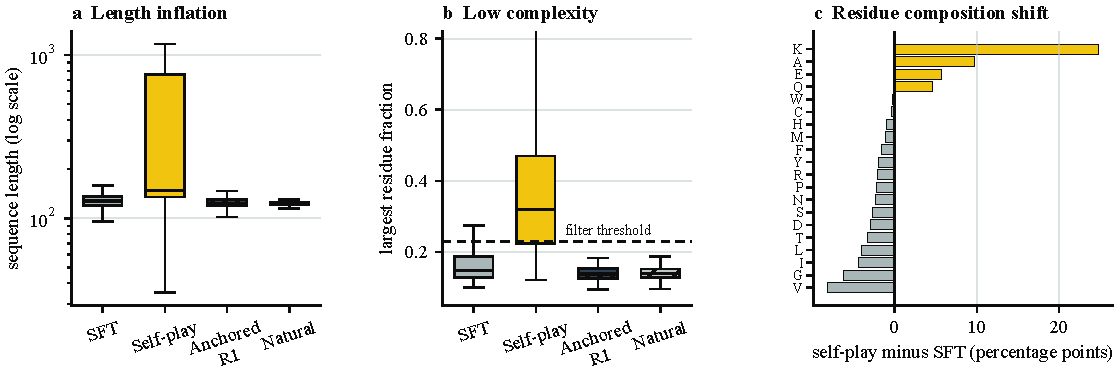
\includegraphics[width=\linewidth]{figures/Figure2_revised.pdf}
\caption{The high-pLDDT policy occupies a pathological sequence
regime. Distributions use evaluation block A; the natural reference contains
571 PF00416 sequences. Boxes show quartiles and medians, and whiskers use the
standard 1.5-IQR rule; outliers are omitted from the drawing but included in
all reported means. Panel c measures residue-frequency change across all
generated residues.}
\label{fig:shortcut}
\end{figure}

This concentration in a small number of amino acids markedly reduced sequence
diversity. Mean residue-distribution entropy fell from 3.752 bits under SFT to
2.763 bits. Equivalently, the most common amino acid accounted for an average
of 37.2\% of each self-play sequence, compared with 17.1\% under SFT and above
the sequence-filter threshold of 23\%. The strong enrichment for lysine, which
is positively charged at pH 7.4, also explains much of the loss of charge
adherence. Among prompts that specified net charge, the mean requested value
was $+14.4$, whereas the self-play generations had a mean computed charge of
$+110.1$.

The most confident self-play output provides a concrete example. ESMFold
assigned it a pLDDT of 93.75, yet the sequence was 194 residues long, contained
68 lysines, and had net charge $+46$. It failed both the specification gate and
the sequence-sanity filters (Appendix Figure~\ref{fig:worked-example}). Thus, self-play increased the optimized proxy by
moving the model toward a narrow and highly charged sequence distribution,
rather than by producing more acceptable conditional generations.

\begin{figure}[b]
\centering
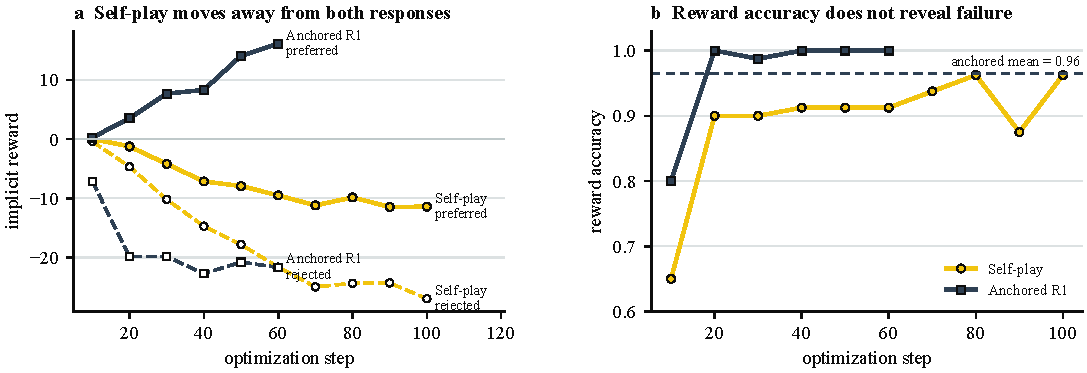
\includegraphics[width=\linewidth]{figures/fig3_training_dynamics.pdf}
\caption{A standard training diagnostic misses the collapse.
Values are taken directly from the trainer states for self-play and anchored
round 1. The anchored mean in panel b is a descriptive reference from that
run, not a decision threshold. Self-play reward accuracy remains high while
both implicit rewards decline.}
\label{fig:training}
\end{figure}

The training diagnostics did not reveal this collapse. DPO requires the
preferred response to outrank the rejected response, but does not require
either response to become more likely in absolute terms
\citep{rafailov2023dpo}. During self-play, the logged implicit reward of the
preferred responses fell from 0.02 to $-11.40$, while that of the rejected
responses fell more rapidly, from $-0.39$ to $-26.95$. The resulting margin therefore increased; after an initial logged value of 0.65, reward accuracy remained between 0.875 and 0.963, even as generation quality deteriorated. High reward accuracy indicated that
the model had learned the pairwise ordering; it did not indicate that the
resulting generations remained acceptable. Full training trajectories are
shown in Figure~\ref{fig:training}.


%\subsection{The relative DPO objective hides absolute drift}

%DPO optimizes a difference of policy-to-reference log-probability ratios. For prompt $x$, preferred response $y^+$, rejected response $y^-$, and reference policy $\pi_{\mathrm{ref}}$, define 
%\begin{equation}
%r_\theta(x,y)=\beta\log\frac{\pi_\theta(y\mid x)}
%{\pi_{\mathrm{ref}}(y\mid x)}.
%\end{equation}
%The DPO loss increases the margin $r_\theta(x,y^+)-r_\theta(x,y^-)$
%\citep{rafailov2023dpo}. It does not require either implicit reward to increase in absolute terms.

%That degree of freedom is visible in the training records
%(Figure~\ref{fig:training}a). During self-play, the logged preferred reward fell from 0.02 at step 10 to $-11.40$ at step 100, while the rejected reward fell from $-0.39$ to $-26.95$. Their margin widened even though the policy moved probability away from both sides of the training pairs. Under the anchored intervention, the preferred reward instead rose from 0.27 to 16.10.

%Reward accuracy records only whether the preferred response outranks the rejected response. After step 10, self-play accuracy stayed between 0.875 and 0.963, overlapping the healthy-looking anchored run (Figure~\ref{fig:training}b). It remained high because the ordering was preserved during the joint decline. Reward accuracy was thus internally consistent with the DPO objective but insufficient as a health diagnostic for the generated sequences.



\subsection{Why anchoring helps once, but not repeatedly}

Anchored DPO changed what the model was trained to prefer. In self-play, both
responses in each preference pair were generated by the SFT policy. In
anchored DPO, the preferred response was instead the natural sequence
associated with the prompt, providing a fixed target drawn from the natural
protein distribution. The auxiliary negative-log-likelihood term also directly
encouraged the model to assign higher probability to that natural sequence.
The subsequent recovery in sequence composition and specification adherence is
consistent with these two forms of anchoring. However, the intervention also
increased $\beta$, and all three changes were introduced together. The
experiment therefore cannot determine which component, or combination of
components, produced the recovery.

Round 2 continued to optimize its training objective: the preferred implicit
reward reached 45.57 and the auxiliary negative log-likelihood fell from 0.884
to 0.094 by step 230. Held-out performance nevertheless remained unchanged.
The new negatives were closer to the natural positives, while the positives
themselves supplied no new biological information. Once a property was already
close to the natural target, a pairwise preference between two similar
responses supplied little directional signal for hitting that target more
precisely. 

\paragraph{Actionable takeaways.}
Within the setting studied here, higher pLDDT was not sufficient evidence of improved generation quality. We therefore considered pLDDT-guided optimization successful only when specification adherence and sequence plausibility were also preserved in a matched held-out evaluation. In practice, three diagnostics should be monitored throughout optimization. First, evaluation should use a joint endpoint that requires prompt adherence, sequence-plausibility checks, and the target pLDDT threshold, rather than pLDDT alone. Second, the implicit rewards of both preferred and rejected responses should be tracked separately: increasing reward accuracy can conceal failure when both rewards decline while their margin widens. Third, basic composition statistics, including sequence length, residue entropy, dominant-residue fraction, and net charge, should be inspected for distributional drift. If pLDDT improves while any of these diagnostics deteriorate, optimization should be stopped and the preference construction or objective revised. Natural-positive anchoring was an effective partial repair in our setting, but its benefit did not increase with a second round and should not be assumed to support indefinite iterative refinement.

\section{Discussion}
\label{sec:discussion}

Instruction tuning improved control over protein generation, but optimizing a
single structural-confidence proxy reversed that progress. Self-play DPO found
a high-pLDDT shortcut consisting of long, compositionally biased sequences,
and standard preference-training diagnostics did not expose the resulting
behavioral collapse. Natural-positive anchoring with an auxiliary likelihood
term partially restored acceptable generations, but repeating the intervention
with fresh negatives provided no further benefit.

The central lesson is that predicted structural confidence cannot be
interpreted independently of the intended generation task. Mean pLDDT alone
would have identified self-play DPO as the best-performing model, despite its
substantial loss of specification adherence and sequence sanity. Evaluating
pLDDT jointly with the specification gate and sequence-sanity filters made the
failure immediately visible. More generally, improvement in a biological proxy
should count as progress only when the generated outputs remain within the
conditions that define an acceptable solution.

This study has several limitations. The experiments concern one language model
and one Pfam family, and ESMFold was the only structure predictor used.
Generalization across protein families, model architectures, structure
predictors, and experimentally relevant endpoints remains untested and is the
subject of our ongoing experiments.

Overall, this case demonstrates that successful optimization of a biological proxy need not constitute improvement on the intended design task. Higher predicted confidence should be treated as one component of success, never as success itself.

\bibliographystyle{plainnat}
\bibliography{references}

\appendix
\setcounter{figure}{0}
\renewcommand{\thefigure}{A\arabic{figure}}
\section{Evaluation definitions}
\label{app:criteria}

A generation was counted as a success only if its parsed amino-acid sequence passed the specification gate, passed every sequence
filter, and had mean ESMFold pLDDT at least 70. Percentages use all 260 prompts
as the denominator, including unparseable generations.

\subsection{Specification gate}

The specification gate first required a valid amino-acid sequence and imposed
unconditional PF00416 bounds of 110-155 residues and net charge 4-25. It then
checked every property that appeared in the prompt:
\begin{itemize}
    \item length within $\pm10\%$ of the requested value;
    \item net charge at pH 7.4 within $\pm2$ charge units;
    \item exact cysteine count when the target was at most two, and $\pm1$
    otherwise;
    \item exact stability bin;
    \item hydrophobicity and aggregation-propensity bins either exact or in an
    adjacent ordinal bin (low, moderate, high); and
    \item aggregate constraint score at least 0.70.
\end{itemize}
The hard per-property requirements prevent a good value on one axis from
compensating for a severe error on another. The unconditional bounds apply even
when a prompt omits length or charge.

Sequence-derived properties were calculated with the same feature code used to construct the prompts. Mean hydropathy and the instability index were calculated using Biopython \citep{cock2009biopython}, following the Kyte--Doolittle scale \citep{kyte1982gravy} and the Guruprasad method \citep{guruprasad1990instability}, respectively. Aggregation propensity was calculated as the sequence mean of the AGGRESCAN a3v residue scores \citep{sanchezdegroot2005prediction,conchillosole2007aggrescan}. Net charge was computed at pH 7.4 and rounded to the nearest integer before comparison.

\subsection{Sequence-plausibility filters}

A sequence was declared protein-like only if all five checks passed:
\begin{enumerate}
    \item all characters belonged to the 20 canonical amino acids;
    \item length was at least 20 residues;
    \item Shannon entropy of the residue distribution was at least 3.2 bits;
    \item no single residue occupied more than 0.23 of the sequence; and
    \item the longest tandem repeat with period one through five covered no
    more than 0.25 of the sequence.
\end{enumerate}
The dominant-residue threshold was calibrated against the full available
natural reference: all 571 PF00416 sequences passed all five checks at these
thresholds. These filters detect the observed shortcut but do not establish
biological function.

\section{Training and evaluation protocol}
\label{app:protocol}

\subsection{Supervised instruction tuning}

The supervised dataset contained 348{,}867 prompt-sequence pairs derived from
reviewed UniProtKB entries. A prompt specified a random subset of the computed
sequence properties. Protein sequences were grouped with MMseqs2 at 30\%
identity and 80\% coverage before the train-test split, so homologous clusters
were not split across partitions. The PF00416 slice used here contained 311
training and 260 held-out sequences.

Llama-3.1-8B-Instruct was loaded in 4-bit precision and adapted with LoRA rank
32, scale 16, and dropout 0.05. SFT used response-only loss for two epochs, a
learning rate of $2\times10^{-4}$, microbatch size 8, gradient accumulation 2,
and random seed 42. The stored run ended at 21{,}804 optimizer steps.

\begin{figure}[t]
\centering
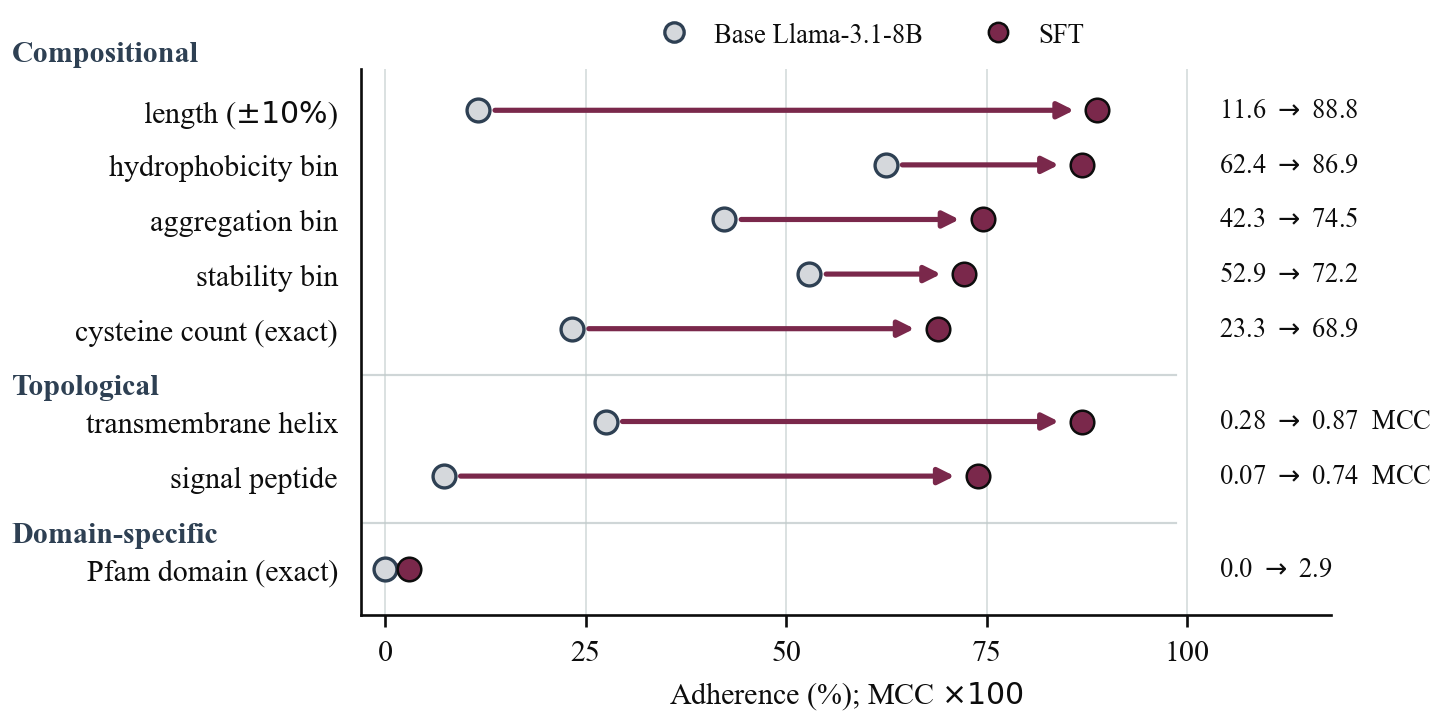
\includegraphics[width=0.94\linewidth]{figures/papera_fig2_adherence.png}
\caption{Instruction tuning improved adherence across the broad held-out
set. Each row is one scored property:
the left marker is the base model and the right marker is the SFT model; the connecting
line shows the gain from fine-tuning. Rows are independent, so percentage and
MCC rows share one axis with MCC $\times 100$. This evaluation used 35{,}115
cluster-separated held-out proteins and precedes the PF00416-specific DPO
experiments.}
\label{fig:papera-adherence}
\end{figure}

\subsection{Preference construction and optimization}

For self-play, candidate generations were first required to pass the same
specification gate and plausibility filters used at evaluation. Surviving
candidates were folded with ESMFold, and higher-pLDDT generations were preferred
to lower-pLDDT generations. The resulting dataset contained 859 pairs from 310
unique prompts. Training used one epoch (107 optimizer steps), DPO
$\beta=0.3$, and no auxiliary likelihood term.

For anchored round 1, the natural sequence associated with the prompt was the
preferred response and a model-generated sequence was rejected. The dataset
contained 929 pairs from 310 unique prompts. The model was trained for 60
optimizer steps with $\beta=0.5$ and an auxiliary negative-log-likelihood term
of weight 1.0. Anchored round 2 began from round 1 and used freshly generated
negatives; its dataset contained 906 pairs from 303 unique prompts. It used the
same objective for 232 specified optimizer steps. In all DPO runs, the frozen
SFT adapter was the reference policy. DPO runs retained LoRA rank 32, scale 16,
dropout 0.05, learning rate $5\times10^{-5}$, microbatch size 2, gradient
accumulation 4, and seed 42.

\subsection{Held-out generation and structural prediction}

All paper results use one sampled generation ($K=1$) for each of the 260
held-out PF00416 prompts. Generation used vLLM, temperature 0.7, nucleus
probability 0.9, maximum 512 new tokens, and seed 99. Each parsed sequence was
evaluated with ESMFold; repeated sequences reused the cached prediction.

Evaluation block A generated the base, SFT, self-play, and anchored round-1
outputs in one process. Block B separately generated SFT, anchored round 1, and
anchored round 2 together. Because stochastic generation and software state can
change the realized samples, no statistical comparison in the paper crosses
these blocks.

\subsection{Statistical analysis}

The primary endpoint was binary at the prompt level. We report counts,
percentages, and two-sided 95\% Wilson score intervals for individual success
rates. For matched policies evaluated on the same prompts, we used the exact
two-sided McNemar test, equivalently a two-sided binomial test on discordant
pairs. These tests are descriptive analyses of the observed evaluation sets;
no prospective power calculation or multiplicity correction was performed.

\section{A worked example of the self-play failure}
\label{app:worked}

The highest-confidence self-play generation is described in
Section~\ref{sec:failure}. Its predicted structure explains why ESMFold scored
it so highly. A lone
helix has almost no tertiary contacts to place, so there is little for a
structure predictor to be uncertain about. Confidence is in fact highest where
the sequence is least protein-like: mean pLDDT rises from 86.3 over the first
20 residues to 96.5 over the last 20, which are almost entirely lysine. Figure~\ref{fig:worked-example} shows this generation alongside the other three
systems on the same prompt.

\begin{figure}[h]
\centering
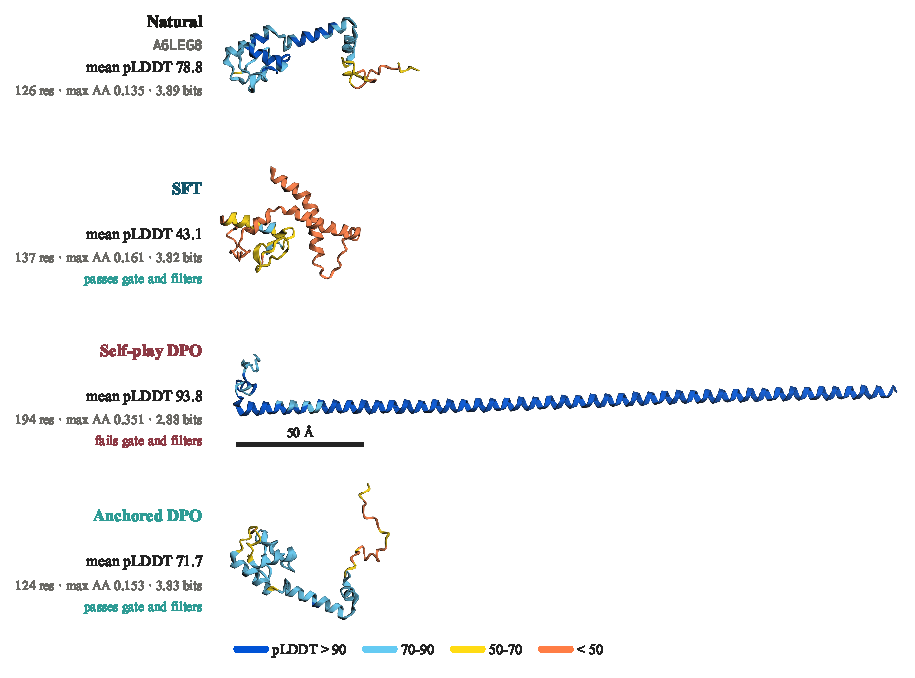
\includegraphics[width=\linewidth]{figures/fig_worked_example.pdf}
\caption{The most confident self-play output, shown with the other systems for
the same held-out prompt (\texttt{A6LEG8}: 126 residues, 1 cysteine, stable, low
hydrophobicity, PF00416). All four structures share one camera and one origin,
so lengths are directly comparable; chains run N to C and are coloured by
per-residue ESMFold confidence. Self-play is the only arm above pLDDT 90 and the
only one that fails the specification gate and the sequence filters. Records are
from evaluation block A.}
\label{fig:worked-example}
\end{figure}

\section{Natural-sequence calibration}

The available natural reference comprised 571 PF00416 sequences: 311 in the
training slice and 260 in the held-out slice. Their mean length was 122.85
residues and their mean ESMFold pLDDT was 78.03. Of these sequences, 566
(99.1\%) had pLDDT at least 70. Mean residue-distribution entropy was 3.890
bits, and the mean dominant-residue fraction was 0.142. All 571 passed the
reported sequence-plausibility filters. This calibration shows that the
filters are compatible with the available natural family members; it does not
make the filters a general definition of naturalness.

\section{Use of generative tools}

A large-language-model writing assistant was used to help reorganize and edit
the manuscript and to assist with figure styling. The authors checked the
reported numerical claims, analyses, citations, and final text against the
stored experimental artifacts and primary sources. The assistant was not used
to generate experimental data or to select the reported results.

\section{Ethical and scientific scope}

This computational study used reviewed protein records and generated amino-acid
sequences; it involved no human participants or animal experiments. No generated
sequence was experimentally validated. The reported pLDDT values and filters
must therefore not be interpreted as evidence that a sequence folds, functions,
or is safe to synthesize.

\end{document}